\part{Comparison} \label{part:Comparison and implementation}

\chapter{Comparisons and implementations}

This chapter will analyze the characteristics of the three algorithms on different real-world data sets. Taking into account the differences between instances (N) and dimension (M), 6 data sets with different N and M will be tested. The code will test the AUC values of the algorithms, and first analyze the individual variables. Then, analyze the variables that affect each other according to the generated heatmap. Finally, this work will take 5 representative values from each variable of each algorithm, use grid search algorithm to find the parameters that each algorithm performs best on the same data set. Analyze the performance difference of $R_{NX}$ curve.\\

\noindent As discussed above, in order to draw the conclusions in a convincing way, This work will examine the three algorithms' quality on several real-world data sets with different N and M, base on the neighborhood-based DR performance criteria discussed above. there are six public databases: Iris, Wine, Breast Cancer Wisconsin Diagnostic (BCW), the Olivetti faces (Oliv), Optical Recognition of Handwritten Digits test set (Digits) and Labeled Faces in the Wild face recognition(LFW). The instance and dimension information of datasets are shown below:\\

\begin{center}
\begin{tabular}{|c|c|c|}% 通过添加 | 来表示是否需要绘制竖线
\hline  % 在表格最上方绘制横线
Datasets & Number of instances & Number of dimensions\\
\hline  %在第一行和第二行之间绘制横线
Iris & 150 & 4\\
\hline  %在第一行和第二行之间绘制横线
Wine & 178 & 13\\
\hline  %在第一行和第二行之间绘制横线
Oliv & 400 & 4096\\
\hline  %在第一行和第二行之间绘制横线
BCW & 569 & 30\\
\hline  %在第一行和第二行之间绘制横线
Digits & 1797 & 64\\
\hline  %在第一行和第二行之间绘制横线
LFW & 13233 & 5749\\
\hline % 在表格最下方绘制横线
\end{tabular}\\
\end{center}
\\

\noindent When we are analyzing the result, we should consider that the high-dimensional sphere was modeled by probability graph, the three DR algorithms adapts its "distance" concept to changes in regional density in the data set. As a result, it naturally expands dense clusters and shrinks sparse clusters, making the clusters roughly uniform in size. It also makes it difficult to see the relative size of clusters in the result graph, and the distance between clusters in low dimensions does not represent directly the distance between clusters in high dimensions.

\section{Grid search algorithm}

Grid search is a parameter adjustment method, with exhaustive strategy: among all the predetermined parameter selections, through looping and trying every possibility, the best performing parameter is the final result. The principle is only in one part. Take this thesis's work as an example. Each algorithm selects the four most important parameters, and each parameter takes 5 typical values. All possibilities are listed, which can be expressed as a 5*5*5*5 four-dimensional table. Each numerical combination is a grid, and the cycle process is like traversing and searching in each grid, so it is called grid search. As for this work, the code will go though all combination of parameters and return the best parameters considering neighborhood-based DR performance criteria.

\section{t-SNE}
There are 4 most important parameters for t-SNE, the ideas of each parameters are: 

\begin{enumerate}[1)]
\item $perplexity$: number of nearest neighbors for each point
\item $n\_iter$: maximum number of iterations for optimization
\item $early\_exaggeration$: the tightness inside clusters and the distance inbetween
\item $min\_grad\_norm$: the threshold for stopping the optimization 
\end{enumerate}\\



\subsection{$perplexity$}

\noindent $perplexity$ represent the number of neighbors each point t-SNE considers. It explains how to maintain a balance between the local and global aspects of the data. The perplexity value has a complex effect on the generated pictures, but the performance of SNE is quite reliable for changes in complexity, and the typical value of perplexity is between 5 and 50\cite{ref9}. Also, since the perplexity means the number of the neighbors, it should not be higher than the total number of data points.\\

\noindent We can try different potential perplexity values in datasets with different instances. At the same time, since the algorithm using stochastic method, the parameter $random\_state$ is set to 1. This parameter determines the random number generator so that it pass an int mark for reproducible results across multiple function calls. After examining it on the first dataset Iris, we get the figures below. For comparing visualization quality on the dataset, From this result, the experiment colored each node with the information of its label in the visualized low-dimensional graph:

\begin{figure}[H]
\centering  %图片全局居中
% \subfigure[name1]
{
\label{Fig.sub.1}
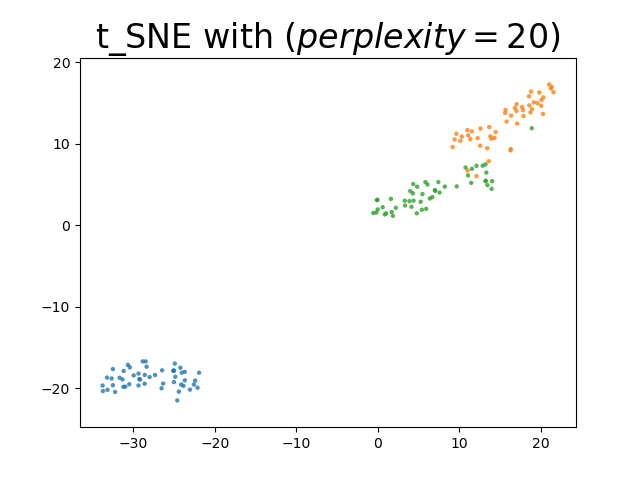
\includegraphics[width=7cm,height=4cm\textwidth]{images/image_comparison_tsne_perp20.png}}
% \subfigure[name2]
{
\label{Fig.sub.2}
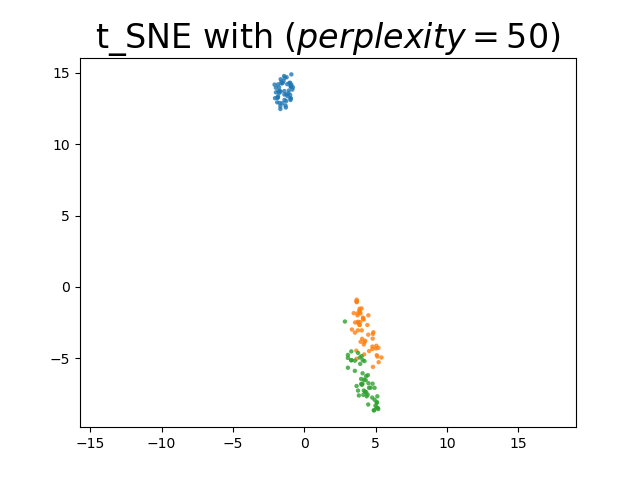
\includegraphics[width=7cm,height=4cm\textwidth]{images/image_comparison_tsne_perp50.png}}
% \caption{LD result for t-SNE with perplecity 20 and 50}
% \label{LD result for t-SNE with n_iter 300 and 500}
% \end{figure}

% \begin{figure}[H]
\centering  %图片全局居中
% \subfigure[name1]
{
\label{Fig.sub.1}
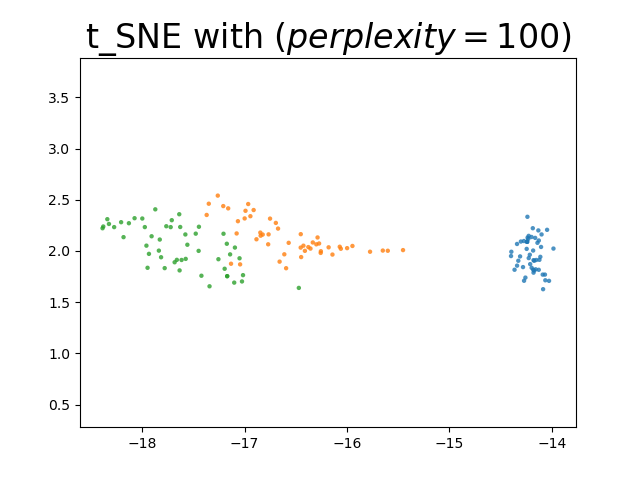
\includegraphics[width=7cm,height=4cm\textwidth]{images/image_comparison_tsne_perp100.png}}
% \subfigure[name2]
{
\label{Fig.sub.2}
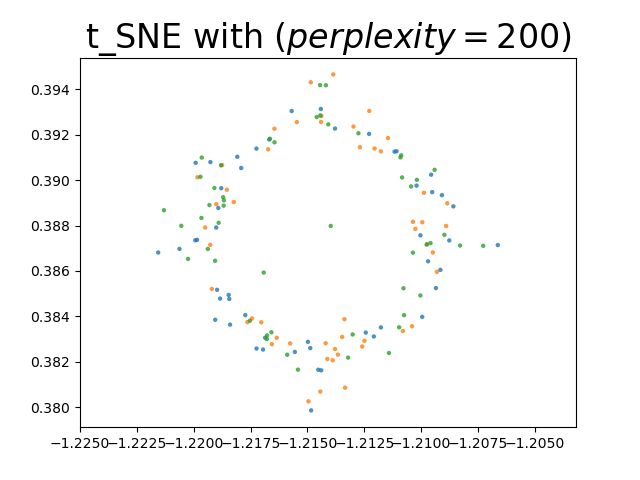
\includegraphics[width=7cm,height=4cm\textwidth]{images/image_comparison_tsne_perp200.png}}
\caption{LD result for t-SNE with different perplecity}
% \label{Fig.main}
\end{figure}


\noindent In the figure, we can see that when the value is in the range of 5-50, clusters are well distinguished. Considering that the number of instances of the dataset is only 150, when the value is 100, the clusters begin to merge. When the perplexity = 200, it is difficult to distinguish different clusters. Considering the experimental results on each dataset and the strategy of the search about the optimal number of neighbor from K nearest neighbour algorithm\cite{ref12}, we can simply set perplexity to $n^{0.5}$, where n stand for number of instances. \\

\noindent At the same time, the $AUC$ value for the result with these parameters are 0.731, 0.658, 0.654, -0.004 separately. These $AUC$ values verifies the previous observations. As for the last one, it has a big difference between others and also the only minus result. With the definition of the $R_{NX}$ curve $R_{NX} (K) = ((N − 1)Q_{NX} (K) − K) /(N − 1 − K)$. This is because the K is higher than N in the formula. The $Q_{NX}$ on the numerator is relative small since the normalization term is largest and denominator is a negative number, we then have a minus result.

\subsection{$n\_iter$}

\noindent $n\_iter$ is the maximum number of iterations for the algorithm. The graph observed above are all generated with 1000 iteration which is the default value of $n\_iter$. In principle, the higher $n\_iter$ gives the better result. However, it may be very time consuming when it comes to big dataset. In contrast, if $n\_iter$ is too small, the algorithm does not have enough iteration to generate the convincing clusters in LD. The most important thing is to reach a stable configuration. The figure shows how the result changes with $n\_iter$ grows in Digits dataset as above:

\begin{figure}[H]
\centering  %图片全局居中
% \subfigure[name1]
{
\label{Fig.sub.1}
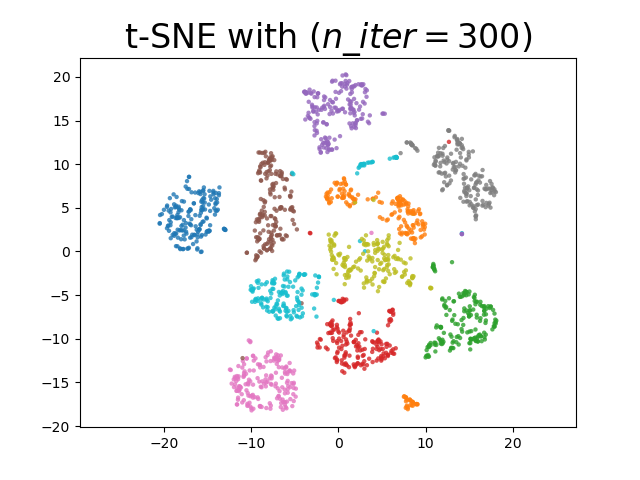
\includegraphics[width=7cm,height=4cm\textwidth]{images/t-sne/tsne_niter_300.png}}
% \subfigure[name2]
{
\label{Fig.sub.2}
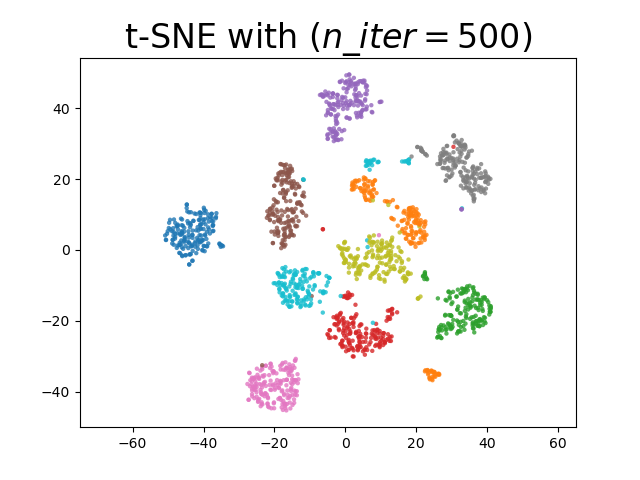
\includegraphics[width=7cm,height=4cm\textwidth]{images/t-sne/tsne_niter_500.png}}
% \caption{LD result for t-SNE with n\_iter 300 and 500}
% \label{Fig.main}
% \end{figure}

% \begin{figure}[H]
\centering  %图片全局居中
% \subfigure[name1]
{
\label{Fig.sub.1}
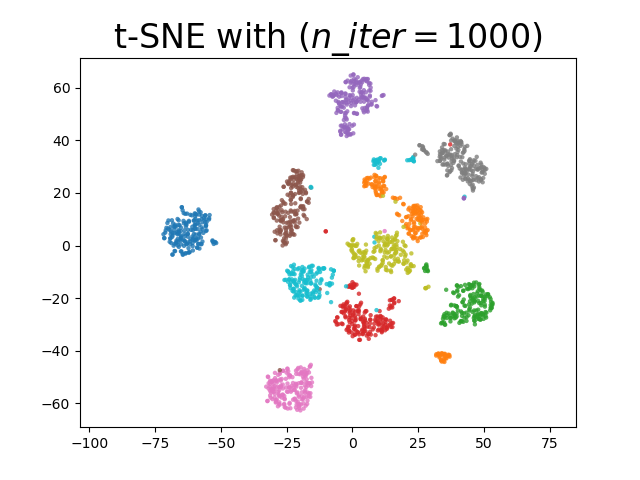
\includegraphics[width=7cm,height=4cm\textwidth]{images/t-sne/tsne_niter_1000.png}}
% \subfigure[name2]
{
\label{Fig.sub.2}
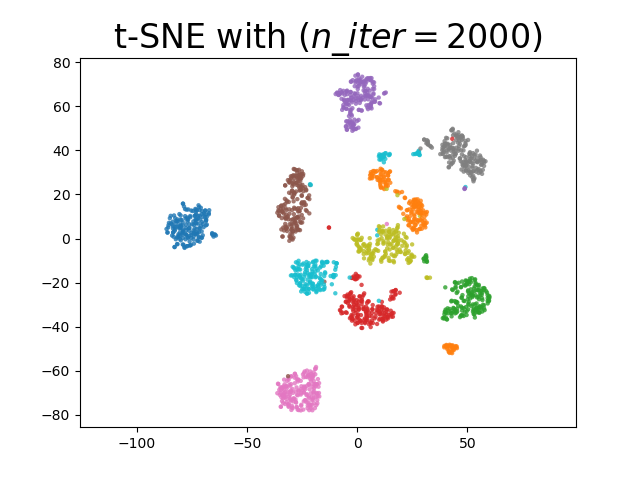
\includegraphics[width=7cm,height=4cm\textwidth]{images/t-sne/tsne_niter_2000.png}}
\caption{LD result for t-SNE with different n\_iter}
% \label{Fig.main}
\end{figure}

\noindent From the figure, we can easily observe that the more iterations, the more well identified for clusters. These four $n\_iter$ generate $AUC$ values for 0.489, 0.526, 0.533, 0.536 separately, which verified the previous conclusion.

\subsection{$min\_grad\_norm$}

This parameter is the threshold of gradient norm to determine when the optimization will be stopped. If the norm is less than the setting value, the gradient descent of Kullback-Leiber divergence will stop. Considering the default number of this parameter is small enough, after examining its potential values, the accuracy is promised if it is set to a relative small value. When it becomes too big, gradient descent may not even find out the local minimum.

\subsection{$early\_exaggeration$}

$ early\_exaggeration $ is a technique in which all $p_{ij}$ are multiplied and "exaggerated" in the early stages of optimization by multipling all $p_{ij}$s a fixed number in the initial stages of the optimization. This means that almost all of the $q_{ij}$ ’s, which still add up to 1, are much too small to model their corresponding $p_{ij}$ ’s. The result of this is to force the value of $q_ {ij}$ to be more concentrated on the larger $ p_{ij} $s, especially for closer points, thereby making the earlier clusters more tightly bound together This creates a lot of relatively empty space in the map, which makes it much easier for the clusters to move around relative to one another in order to find a good global organization\cite{ref13}. By doing that, it can control the closeness of clusters in high-dimensional space and the distance between them in low-dimensional space. For larger values, the space between natural clusters will be larger in the embedded space.


\subsection{Relations between parameters}

The code of examination also generates a series of heatmaps to show the relationship of each parameter pair. The algorithm also generates a series of heatmaps to show the relationship of each parameter pair. Heatmap represents the effect of one parameter change on another parameter when other parameters take default values. According to the operation of t-SNE on 6 data sets, :

\subsubsection{$early\_exaggeration$ and $n\_iter$:}

The figures below shows the heatmap between $early\_exaggeration$ and $n\_iter$ for each dataset:


\begin{figure}[H]
\centering  %图片全局居中
\subfigure[Iris]
{
\label{Fig.sub.1}
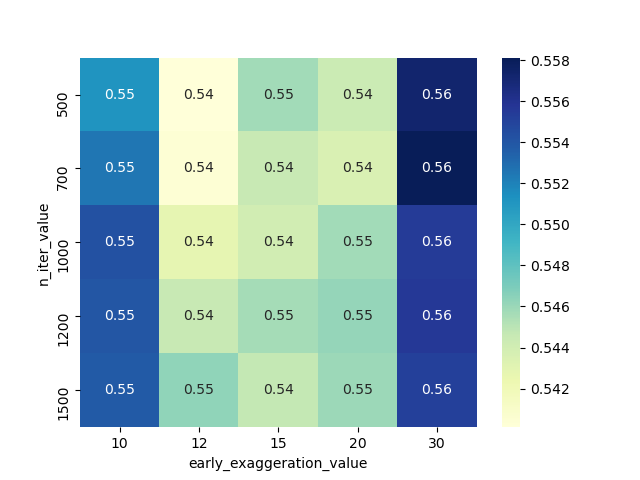
\includegraphics[width=7cm,height=4.5cm\textwidth]{images/t-SNE_conparison/Iris_auc_value_n_iter_value_early_exaggeration_value_heatmap.png}}
\subfigure[Wine]
{
\label{Fig.sub.2}
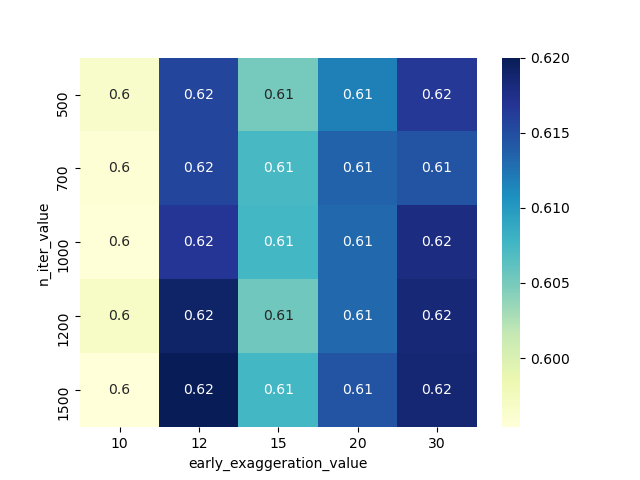
\includegraphics[width=7cm,height=4.5cm\textwidth]{images/t-SNE_conparison/Wine_auc_value_n_iter_value_early_exaggeration_value_heatmap.png}}
% \label{Fig.main}
% \end{figure}

% \begin{figure}[H]
\centering  %图片全局居中
\subfigure[Oliv]
{
\label{Fig.sub.1}
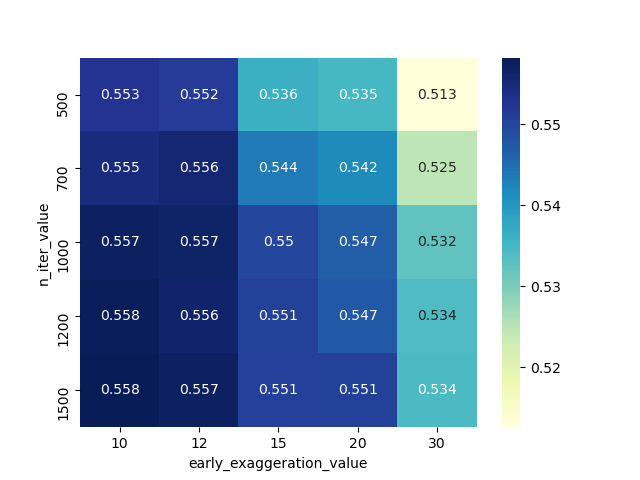
\includegraphics[width=7cm,height=4.5cm\textwidth]{images/t-SNE_conparison/Oliv_auc_value_n_iter_value_early_exaggeration_value_heatmap.png}}
\subfigure[BCW]
{
\label{Fig.sub.2}
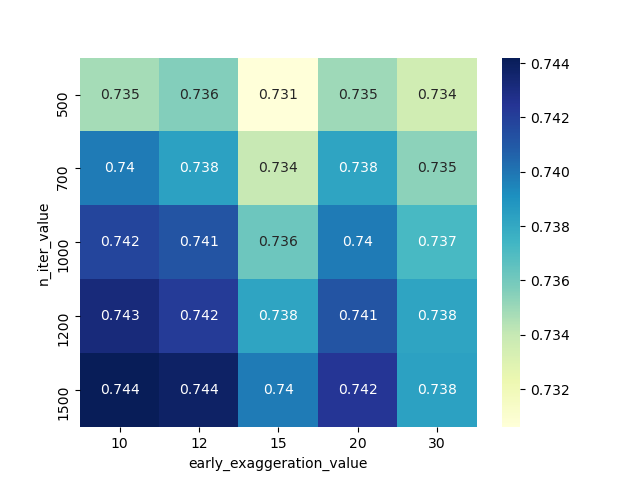
\includegraphics[width=7cm,height=4.5cm\textwidth]{images/t-SNE_conparison/BCW_auc_value_n_iter_value_early_exaggeration_value_heatmap.png}}
% \label{Fig.main}
% \end{figure}
% \begin{figure}[H]
\centering  %图片全局居中
\subfigure[Digits]
{
\label{Fig.sub.1}
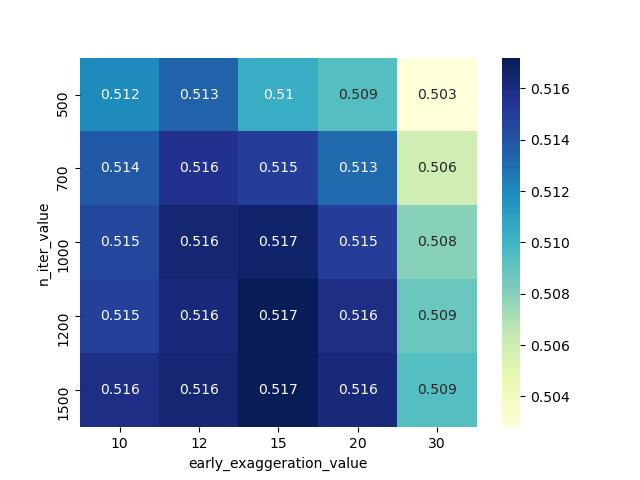
\includegraphics[width=7cm,height=4.5cm\textwidth]{images/t-SNE_conparison/Digit_auc_value_n_iter_value_early_exaggeration_value_heatmap.png}}
\subfigure[LFW]
{
\label{Fig.sub.2}
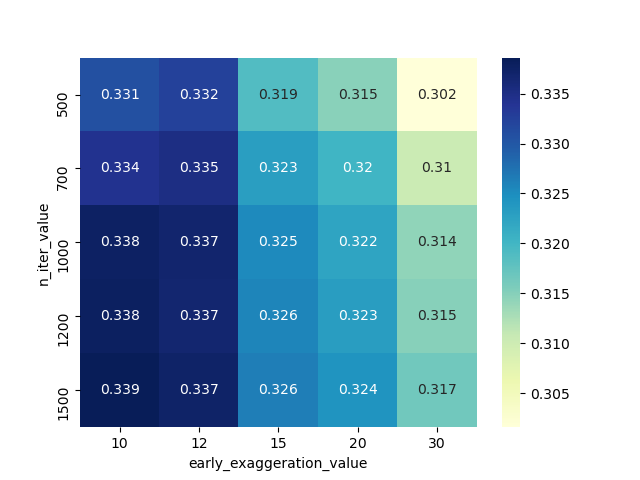
\includegraphics[width=7cm,height=4.5cm\textwidth]{images/t-SNE_conparison/LFW__auc_value_n_iter_value_early_exaggeration_value_heatmap.png}}

\centering
\caption{$early\_exaggeration$ and $n\_iter$ on different dataset}
% \label{}
\end{figure}

\noindent It is easy to find that when $early\_exaggeration$ goes smaller and $n\_iter$ goes larger, the performance of t-SNE is the better. When these two parameters come to smallest and largest of the range separately, the AUC value is the best. Except on two small dataset (Iris and Wine), where the better result is almost as good as other values with the difference of AUC to other values less than 0.01. This make sense since larger $early\_exaggeration$ force clusters to move around relative to one another in order to find a good global structure. With the number of iteration increase, there are higher probability for algorithm to reach a stable configuration.

% \subsubsection{$early\_exaggeration$ and $perplexity$:}
% % \subsubsection{$perplexity$ and $n\_iter$:}

\subsubsection{Running time:}

As in the previous theoretical analysis,  It is easy to find that running time increase with $perplexity$ and $n\_iter$ affect the running time the most. The time increases significantly with these two variables independently with the same trend on 6 data sets. Take digits dataset as an example, there are heatmaps for these two parameters with others:

\begin{figure}[H]
\centering  %图片全局居中
% \subfigure[$min\_grad\_norm$ and $n\_iter$]
{
\label{Fig.sub.1}
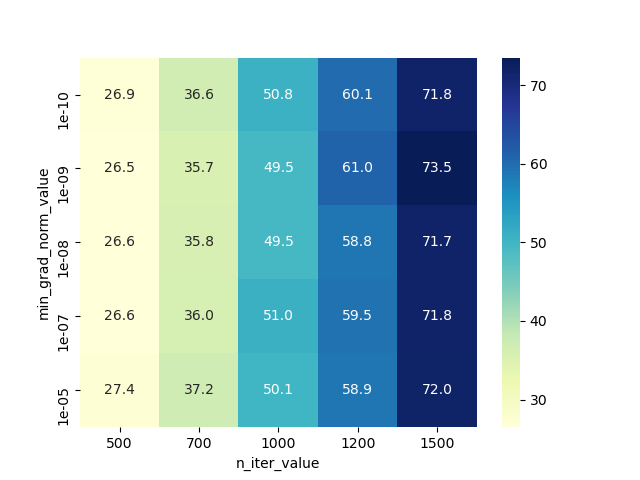
\includegraphics[width=4.5cm,height=4.5cm\textwidth]{images/t-sne/Digit_elapsed_time_min_grad_norm_value_n_iter_value_heatmap.png}}
% \subfigure[$perplexity$ and $early\_exaggeration$]
{
\label{Fig.sub.2}
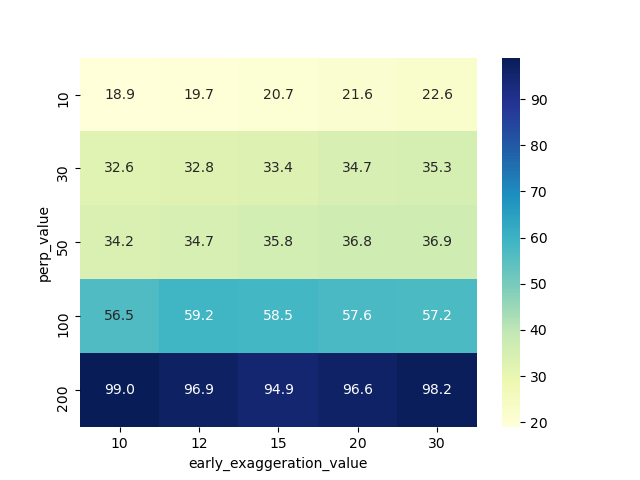
\includegraphics[width=4.5cm,height=4.5cm\textwidth]{images/t-sne/Digit_elapsed_time_perp_value_early_exaggeration_value_heatmap.png}}
% \subfigure[$perplexity$ and $n\_iter$]
{
\label{Fig.sub.3}
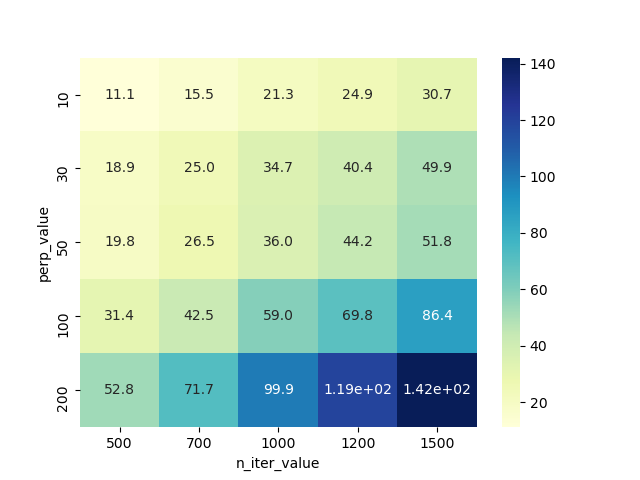
\includegraphics[width=4.5cm,height=4.5cm\textwidth]{images/t-sne/Digit_elapsed_time_perp_value_n_iter_value_heatmap.png}}
\centering
\caption{Running time for perplexity and n\_iter on Digits dataset with other parameters set to default }
% \label{Fig.main}
\end{figure}

\section{UMAP}
There are 4 most important parameters for UMAP, the ideas of each parameters are:

\begin{enumerate}[1)]
\item $n\_neighbors$: The size of local neighborhood like perplexity for t-SNE
\item $min\_dist$: The effective minimum distance between embedded points
\item $spread$: The effective scale of embedded points
\item $negative\_sample\_rate$: Number of negative samples for per positive sample
\end{enumerate}\\

\subsection{$n\_neighbors$}

The size of the local neighborhood used for manifold approximation.  Its default value is 15 instead of 30 for $perplexity$ in t-SNE. This make sense since the definition of K is $k = 2^{\sum_i p_{ij}}$ where $p_{ij} = p_{i\mid j} + p_{j\mid i} - p_{i\mid j}p_{j\mid i}$ without the log 2 function in perplexity as $perplexity = 2^{-\sum_i p_{i \mid j} \log_2 p_{i \mid j} }$. \\

\noindent The changes allows this parameter controls how UMAP balances local versus global structure in the data.It does this by constraining the size of the local neighborhood UMAP will look at when attempting to learn the manifold structure of the data. This means that low values of $n\_neighbors$ will force UMAP to concentrate on very local structure, while large values will push UMAP to look at larger neighborhoods of each point when estimating the manifold structure of the data, losing fine detail structure for the sake of getting the broader of the data. Also, since the $n\_neighbors$ means the number of the neighbors, it should not be higher than the number of data points.\\

\noindent We can try different potential perplexity values in datasets with different instances. Same as t-SNE, in order to avoid the effect of stochastic for each round, the parameter is $random_stateis$ set to 1. After examining it on the dataset Digits, we get the figures below:

\begin{figure}[H]
\centering  %图片全局居中
% \subfigure[name1]
{
\label{Fig.sub.1}
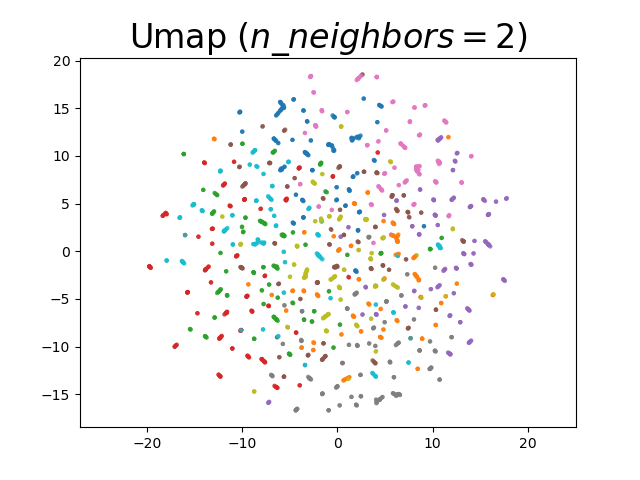
\includegraphics[width=7cm,height=4cm\textwidth]{images/umap/umap_digit_n_neighbor_2.png}}
% \subfigure[name2]
{
\label{Fig.sub.2}
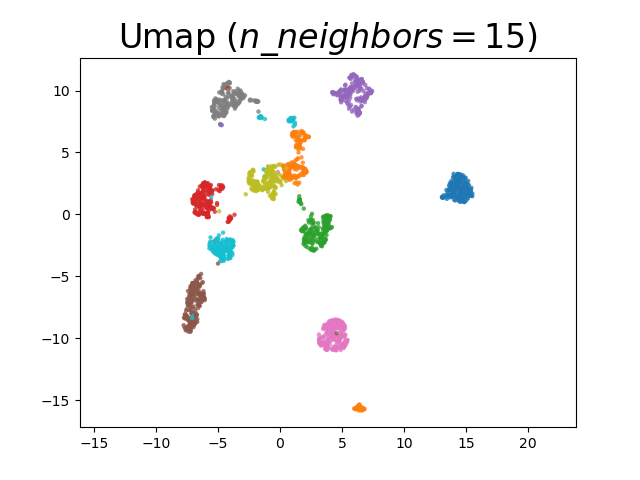
\includegraphics[width=7cm,height=4cm\textwidth]{images/umap/umap_digit_n_neighbor_15.png}}
% \caption{LD result for UMAP with n\_iter 2 and 15}
% \label{Fig.main}
% \end{figure}

% \begin{figure}[H]
% \subfigure[name1]
{
\label{Fig.sub.1}
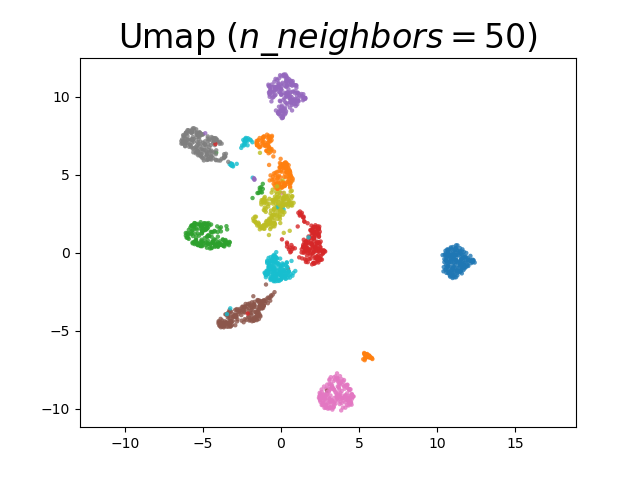
\includegraphics[width=7cm,height=4cm\textwidth]{images/umap/umap_digit_n_neighbor_50.png}}
% \subfigure[name2]
{
\label{Fig.sub.2}
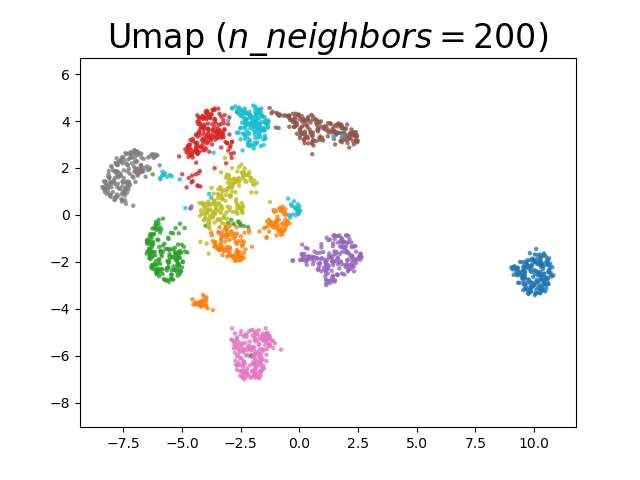
\includegraphics[width=7cm,height=4cm\textwidth]{images/umap/umap_digit_n_neighbor_200.png}}
\caption{LD result for UMAP with different n\_iter}
% \label{Fig.main}
\end{figure}

\noindent These values of $n\_neighbors$ lead to AUC values for 0.391, 0.449, 0.437, 0.431 seperately. As we can observe from the figure, with the number of $n\_neighbors$ increases, when constructing graphical representations of high-dimensional data, UMAP connects more and more adjacent points, which leads to a projection that more accurately reflects the global structure of the data. When it is a very low value at 2, it focus on the local structure completely. \\

\subsection{$min\_dist$}

The $min_dist$ parameter controls how tightly UMAP is allowed to pack points together. It, quite literally, provides the minimum distance apart that points are allowed to be in the low dimensional representation. This means that low values of $min_dist$ will result in clumpier embeddings. Larger values of $min_dist$ will prevent UMAP from packing point together and will focus instead on the preservation of the broad topological structure instead.\\

\noindent UMAP uses the family of curves $1 / (1+a*y^(2b))$ for modelling distance probabilities in low dimensions, not exactly Student t-distribution but very-very similar, without normalizatiom. As the formula mentioned in the theoretical part, the $min_dist$ determine the $a$ and $b$ for the curve directly:

\begin{equation*}
    {q_i_j} = (1 + a(y_i - y_j)^{2b} )^{-1} = \left\{
             \begin{array}{lr}
             1 &  y_i - y_j \leq min\_dist\\
             e^{-(y_i - y_j)-min\_dist}, & y_i - y_j \textgreater min\_dist 
             \end{array}
\right.
\end{equation*}

\noindent Here below are figures with different $min\_dist$ with the Digit dataset as above:

\begin{figure}[H]
\centering  %图片全局居中
% \subfigure[name1]
{
\label{Fig.sub.1}
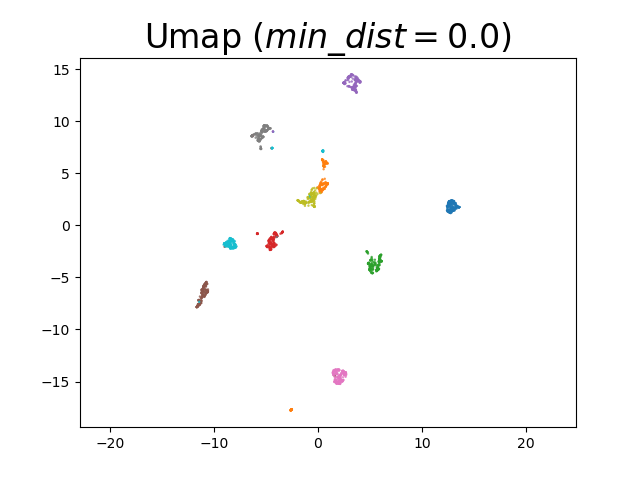
\includegraphics[width=7cm,height=4cm\textwidth]{images/umap/umap_min_dist_0.0.png}}
% \subfigure[name2]
{
\label{Fig.sub.2}
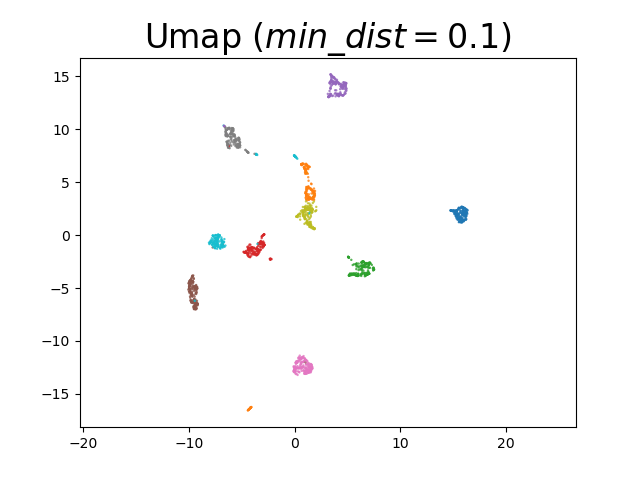
\includegraphics[width=7cm,height=4cm\textwidth]{images/umap/umap_min_dist_0.1.png}}
% \caption{LD result for UMAP with min\_dist 0.0 and 0.1}
% \label{Fig.main}
% \end{figure}

% \begin{figure}[H]
\centering  %图片全局居中
% \subfigure[name1]
{
\label{Fig.sub.1}
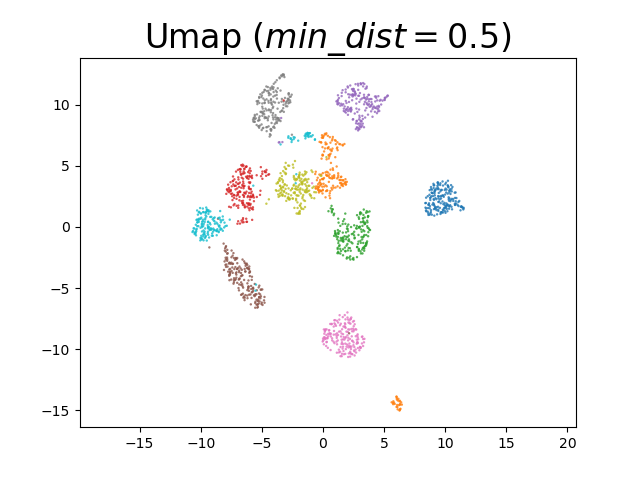
\includegraphics[width=7cm,height=4cm\textwidth]{images/umap/umap_min_dist_0.5.png}}
% \subfigure[name2]
{
\label{Fig.sub.2}
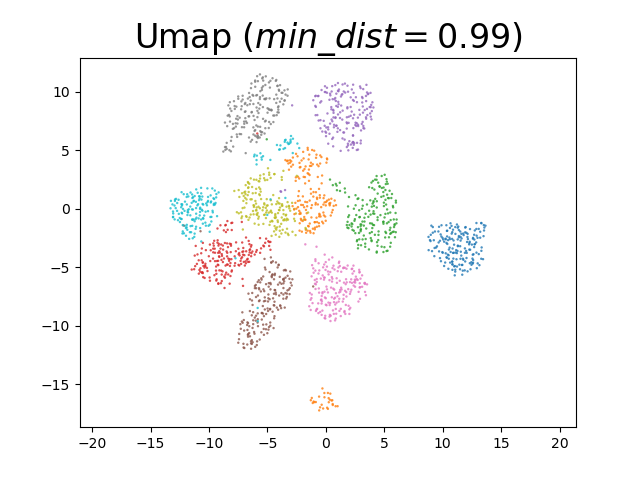
\includegraphics[width=7cm,height=4cm\textwidth]{images/umap/umap_min_dist_0.99.png}}
\caption{LD result for UMAP with different min\_dist}
% \label{Fig.main}
\end{figure}

% 继续把min_dist搞完,之后时spread,参照网页先不考虑两者之间的关系。

\noindent From the figures above, we see that using $min\_dist$=0.0, UMAP can find smaller connected components and clusters in the data, and emphasize these features in the final embedding. As these structures in $min\_dist$ increase, the size of the clusters also increase. These structures are pushed into softer and more general functions, which provide a better overall view of the data without the loss of more detailed topology. 

\subsection{$spread$}

$spread$ control the effective scale of embedded points, which means it determines the scale at which embedded points will be spread out. Whereas increasing spread keeps the shape and boundary of the clusters a bit better. Spread can therefore be used to control the inter-cluster distances to some extent, where as $min\_dist$ controls the size of the clusters.

\subsection{$negative\_sample\_rate$}

This parameter determine the number of negative samples to select per positive sample in the optimization process. Increasing this value will result in greater repulsive force being applied, greater optimization cost, but slightly more accuracy. Here below are figures for different $negative\_sample\_rate$ values:

\begin{figure}[H]
\centering  %图片全局居中
% \subfigure[name1]
{
\label{Fig.sub.1}
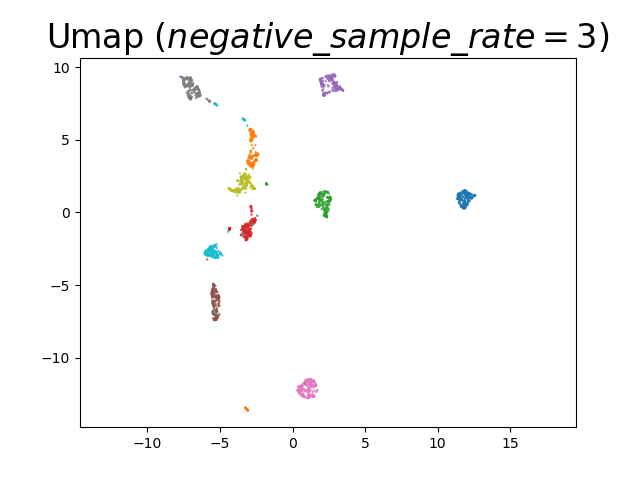
\includegraphics[width=7cm,height=4cm\textwidth]{images/umap/umap_neg_3.png}}
% \subfigure[name2]
{
\label{Fig.sub.2}
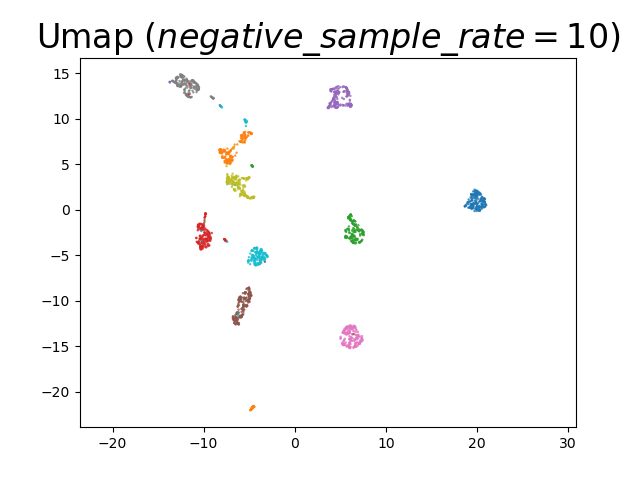
\includegraphics[width=7cm,height=4cm\textwidth]{images/umap/umap_neg_10.png}}
% \caption{LD result for UMAP with min\_dist 0.0 and 0.1}
% \label{Fig.main}
% \end{figure}

% \begin{figure}[H]
\centering  %图片全局居中
% \subfigure[name1]
{
\label{Fig.sub.1}
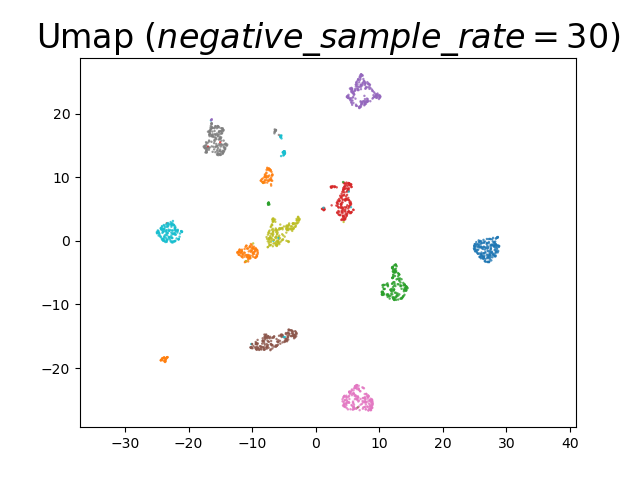
\includegraphics[width=7cm,height=4cm\textwidth]{images/umap/umap_neg_30.png}}
% \subfigure[name2]
{
\label{Fig.sub.2}
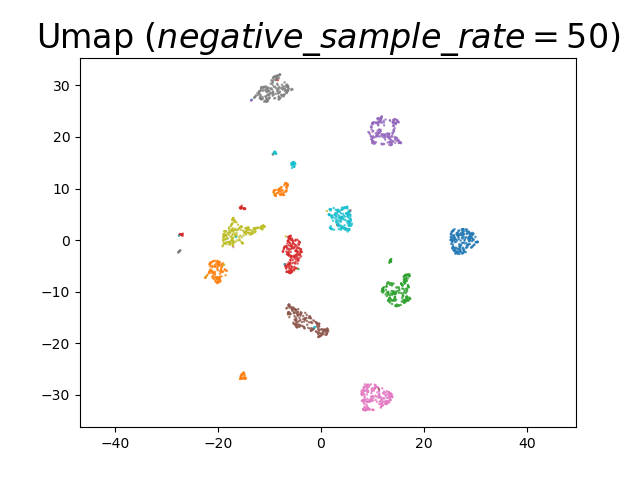
\includegraphics[width=7cm,height=4cm\textwidth]{images/umap/umap_neg_50.png}}
\caption{LD result for UMAP with negative\_sample\_rate}
% \label{Fig.main}
\end{figure}

\noindent As we can observe, the clusters are more well identified with the increase of $negative\_sample\_rate$. As for the result, these four setting of the parameter has $AUC$ values 0.402, 0.425,  0.430, 0.449. At the same time, the running time (second) for each are 4.385, 7.749, 9.552,  25.615,  45.477 separately, which confirmed the previous argument.\\

\subsection{Relationships between algorithms and parameters}

\subsubsection{Running time}

The most obvious finding is that UMAP use much less time than t-SNE to run the code in each dataset. Here below is the comparison between UMAP and t-SNE: 

\begin{figure}[ht]

\centering
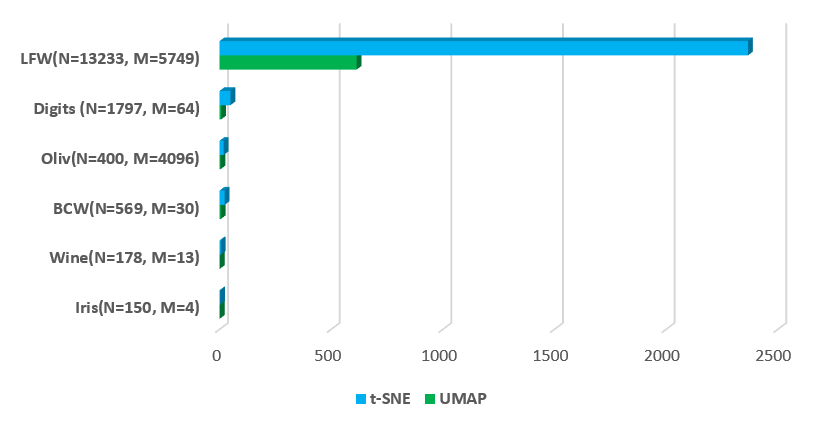
\includegraphics[width=12cm,height=7cm\textwidth]{images/image_time_umap_t-SNE.PNG}
\caption{Time consumption on different dataset for 2 algorithms
}
\label{fig:label}
\end{figure}\\

There are several reasons for this:
\begin{enumerate}[1)]

\item As defined above, the High-dimensional and low-dimensional probability is expressed as $p_{i \mid j} = e^{-\frac{d(x_i,x_j) - \rho}{\sigma_i}}$ with $p_{ij} = p_{i\mid j} + p_{j\mid i} - p_{i\mid j}p_{j\mid i}$ and 
${q_i_j} = (1 + a(y_i - y_j)^{2b} )^{-1}$, which do not apply normalization. Although they have been scaled for the segment [0,1], it turns out that there is no normalization, such as the denominator in the equation of $p_{i \mid j}$. The time for calculating high-dimensional graphs is greatly reduced, because summation or integration is a computationally expensive process. This method is like the Markov Chain Monte Carlo algorithm (MCMC). \\

\item Different with the random normal initialization used by tSNE, UMAP uses the graph laplacian method to assign initial low-dimensional coordinates. This will reduce the UMAP change from iteration to iteration because it is no longer random initialization.\\
   
\subsubsection{The global structure preserved better using UMAP}

With a better global structure visualization result and better AUC acore, UMAP have a better balance betweeb local and global structure.\\

This firstly because of different cost function using Cross-Entropy instead of the KL-divergence. As discussed above, we have:
\begin{equation*}
    C_{EUMAP}(X,d_i_j) = \sum _{j}[-P(X) \log Q(d_i_j) + (1 - P(X)) \log (1-Q(d_i_j))]
\end{equation*}

It can turn out to be:

\begin{equation*}
\begin{aligned}
C_{EUMAP}(X,d_i_j)  &= \sum _{j}[-P(X) \log Q(d_i_j) + (1 - P(X)) \log (1-Q(d_i_j))]\\
&= e^{-X^2} \log \left[ e^{-X^2} (1 + Y^2) \right] + (1 - e^{-X^2}) \log \left[ \frac{ (1 - e^{-X^2})(1 + Y^2)}{Y^2}\right]\\
&\approx e^{-X^2} \log (1 + Y^2) + (1 - e^{-X^2}) \log (\frac{1 + Y^2}{Y^2})
\end{aligned}
\end{equation*}

This leads to the change in the preservation balance of the local-global structure. At a smaller value of $X$, we obtain the same limit as t-SNE, because the second term disappears due to the previous factor, and the logarithmic function is slower than the polynomial function:

\begin{equation*}
\limits X \to 0 :{CE(X,Y) \approx \log (1 + Y^2)} 
\end{equation*}

Therefore, in order to minimize the loss, the Y coordinate is forced to be small, that is, $Y \to 0$. This is exactly the same behavior as t-SNE. However, in the opposite limit of large $X$, the first term disappears and the former factor of the second term becomes 1, we get:

\begin{equation*}
\limits X \to \infty :{CE(X,Y) \approx \log (\frac{1 + Y^2}{Y^2})} 
\end{equation*}

If $Y$ is small, we will get a high penalty due to $Y$ in the logarithmic denominator, so we encourage Y to be large so that the ratio under the logarithm becomes 1, and we get zero penalty. Therefore, we get $Y\to\infty$ at $X\to\infty$, so when moving from high-dimensional space to low-dimensional space, the global distance is preserved.\\

\subsubsection{Relationship between $perplexity$ and $n\_neighbor$}

t-SNE and UMAP both define the high-dimensional probability at a certain distance for observing points as:

\begin{equation*}
p_{ij} \approx e^{-\frac{(x_i - x_j)^2}{2\sigma_i^2}}
\end{equation*}

Here $\sigma$ is the parameter for how many samples can be detected by each other, which is a finite value. This means the data points over the threshold of $\sigma$ will not be considered as a candidate to analyze. Because both tSNE and UMAP are neighbor graph algorithms, the local structure of the graph is retained. However, when $\sigma\to\infty$, every point has a chance to detect every other point, which means, in principle, both t-SNE and UMAP can retain the global structure. However, $\sigma$  is not the hyperparameter of tSNE and UMAP, but as a variable of $perplexity$ and $n\_neigbor$ respectively.\\


% ***** check *****
% Here the figure 6.14 shows how the mean $\sigma$ infected by the $perplexity$ and $n\_neighbor$ hyperparameters.\\

% \begin{figure}[ht]

% \centering
% 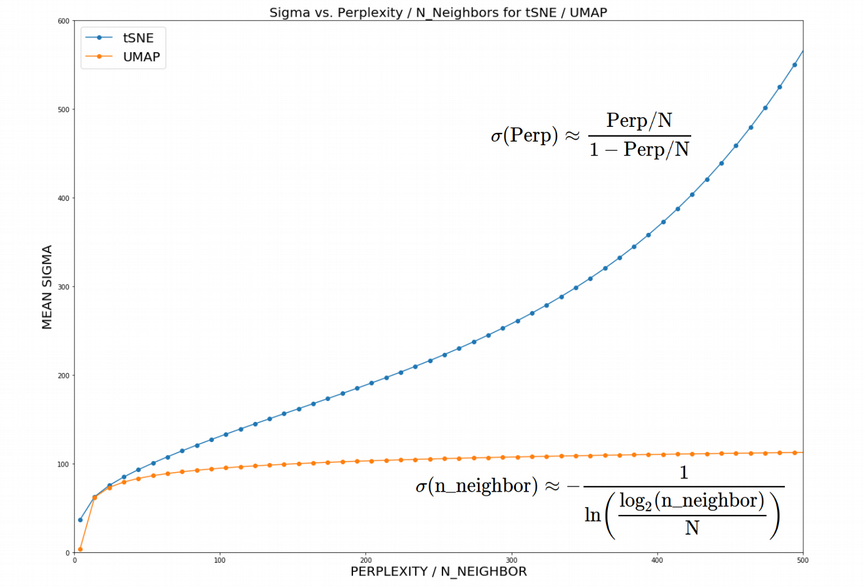
\includegraphics[width=12cm,height=7cm\textwidth]{images/image_sigmma.png}
% \caption{Behavior of mean $\sigma$ as a variable of $perplexity$ and $n\_neighbor$}
% \label{fig:label}
% \end{figure}\\

% ***** check *****\\

We can easily observe that the $n\_neighbor$ hyperparameter is increased, the average sigma of UMAP will soon reach a plateau, while t-SNE is much more sensitive to $perplexity$. When it comes to big $perplexity$, the almost hyperbolic difference of the average $\sigma$ of t-SNE has a huge impact on the gradient of the tSNE cost function (KL difference). In the limit σ→∞, the high-dimensional probability in the above formula becomes 1, which leads to a decrease in the KL divergence gradient.\\

\subsubsection{Relationship between $n\_neighbors$ and $min\_dist$}

From the previous derivation, we can basically draw the conclusion that $n\_neighbors$ change the balance between local and global structure and $min\_dist$ determine the size of the clusters. These two parameters affect the performance of the algorithm the most.\\

The figures below shows the heatmap between $n\_neighbors$ and $min\_dist$ for each dataset, it is easy to find that when $min\_dist$ goes middle of the range around 0.5 and $n\_neighbors$ goes also middle of the range around 50, the performance of UMAP is the best. Except on LFW dataset, where the better result comes from two parameters are set to almost minimum of the range. This may because the size of LFW is 10 to 100 times higher in both instances and dimensions comparing with the rest of the dataset. So the algorithm need to focus more on smaller scale of the structure and keep the size of the clusters relatively small in order to have a better dimension reduction result.  

\begin{figure}[H]
\centering  %图片全局居中
\subfigure[Iris]
{
\label{Fig.sub.1}
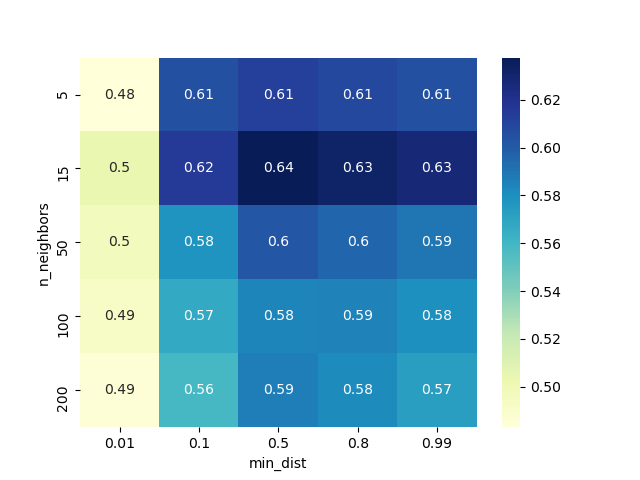
\includegraphics[width=7cm,height=3.5cm\textwidth]{images/umap/comparison/Iris_auc_value_n_neighbors_min_dist_heatmap.png}}
\subfigure[Wine]
{
\label{Fig.sub.2}
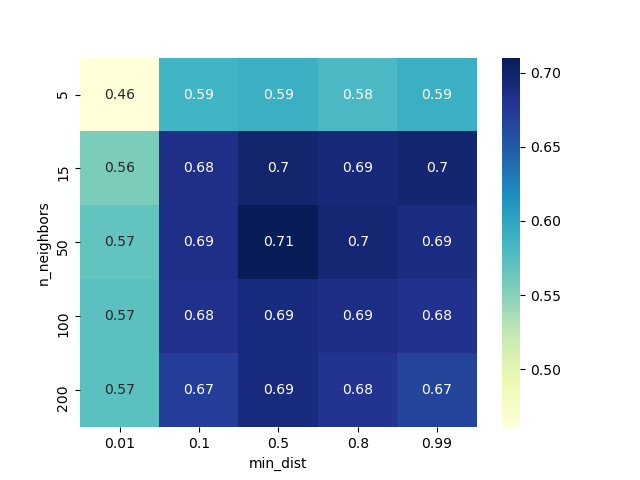
\includegraphics[width=7cm,height=3.5cm\textwidth]{images/umap/comparison/Wine_auc_value_n_neighbors_min_dist_heatmap.png}}
% \caption{LD result for UMAP with n\_iter 2 and 15}
% \label{Fig.main}
% \end{figure}

% \begin{figure}[H]
\centering  %图片全局居中
\subfigure[BCW]
{
\label{Fig.sub.1}
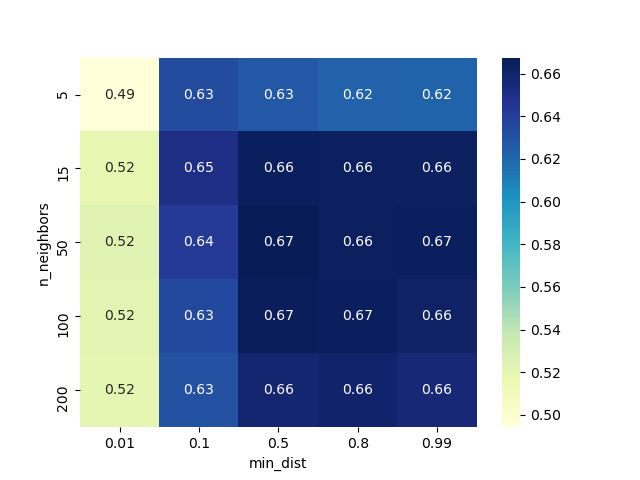
\includegraphics[width=7cm,height=3.5cm\textwidth]{images/umap/comparison/BCW_auc_value_n_neighbors_min_dist_heatmap.png}}
\subfigure[Oliv]
{
\label{Fig.sub.2}
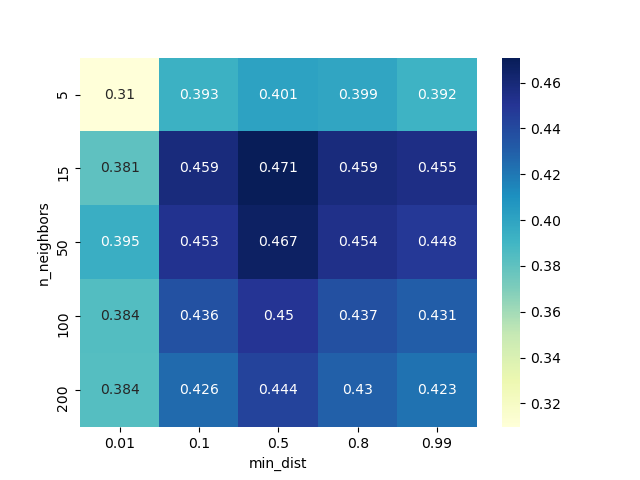
\includegraphics[width=7cm,height=3.5cm\textwidth]{images/umap/comparison/Oliv_auc_value_n_neighbors_min_dist_heatmap.png}}
% \caption{LD result for UMAP with n\_iter 50 and 200}
% \label{Fig.main}
% \end{figure}

% \begin{figure}[H]
\centering  %图片全局居中
\subfigure[Digit]
{
\label{Fig.sub.1}
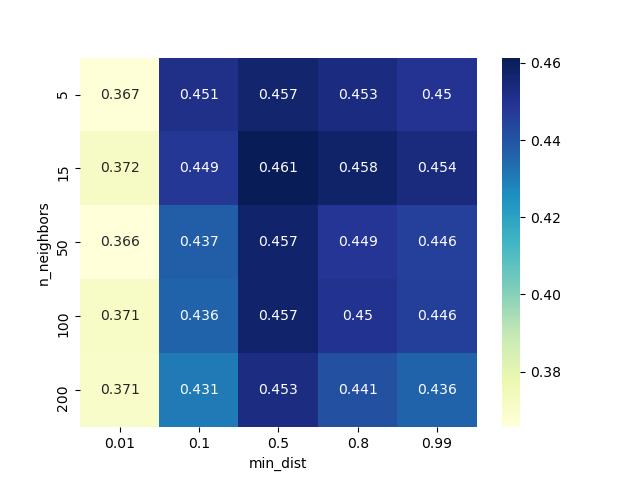
\includegraphics[width=7cm,height=3.5cm\textwidth]{images/umap/comparison/Digit_auc_value_n_neighbors_min_dist_heatmap.png}}
\subfigure[LFW]
{
\label{Fig.sub.2}
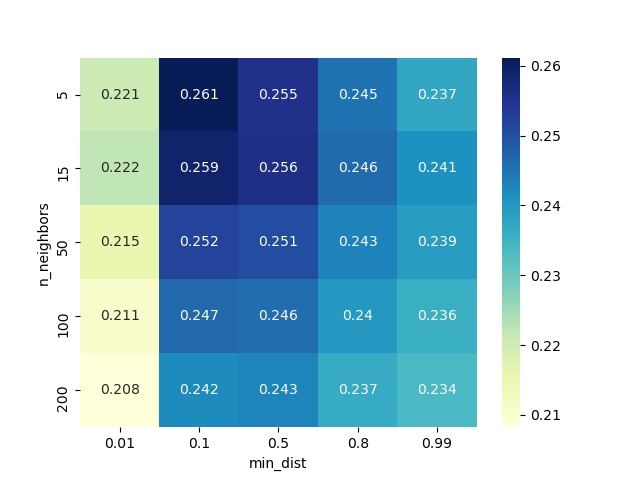
\includegraphics[width=7cm,height=3.5cm\textwidth]{images/umap/comparison/LFW__auc_value_n_neighbors_min_dist_heatmap.png}}
\caption{Heatmap result with different $n\_neighbors$ and $min\_dist$ in different dataset}
% \label{Fig.main}
\end{figure}

\subsubsection{Influence of parameters on running time}

Although UMAP runs faster than t-SNE, there are still differences how each parameter infect the time consumption.  $n\_neighbors$ and $negative\_sample\_rate$ are two most decisive parameters with the increasement of them. Due to space limitations, here will show the time consumption tendency in the heatmap form Digits, which is the representative dataset:

\begin{figure}[H]
\centering  %图片全局居中
% \subfigure[$min\_grad\_norm$ and $n\_iter$]
{
\label{Fig.sub.1}
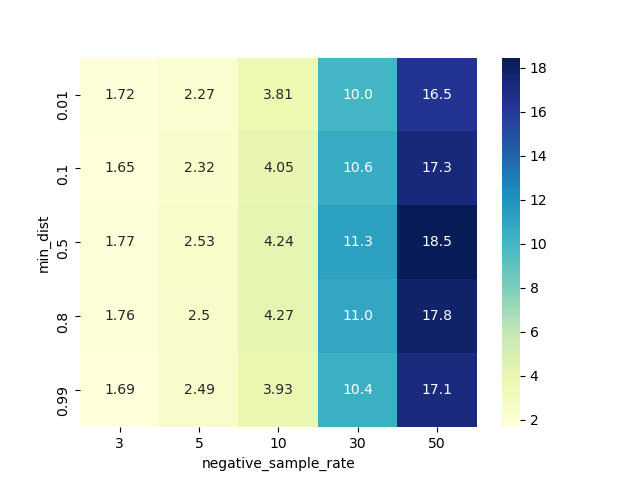
\includegraphics[width=4.5cm,height=4cm\textwidth]{images/umap/comparison/Digit_elapsed_time_min_dist_negative_sample_rate_heatmap.png}}
% \subfigure[$perplexity$ and $early\_exaggeration$]
{
\label{Fig.sub.2}
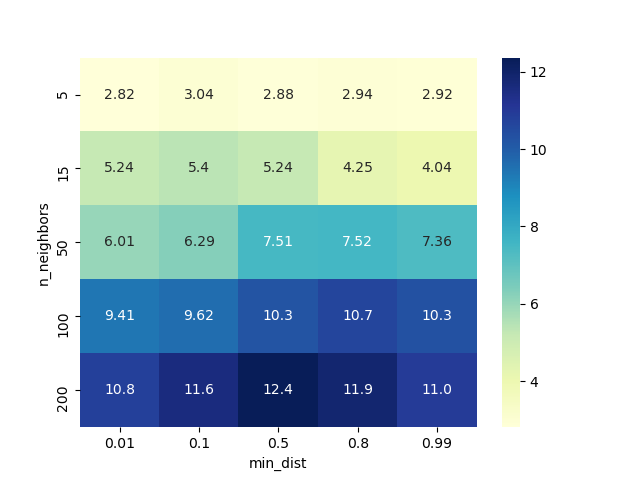
\includegraphics[width=4.5cm,height=4cm\textwidth]{images/umap/comparison/Digit_elapsed_time_n_neighbors_min_dist_heatmap.png}}
% \subfigure[$perplexity$ and $n\_iter$]
{
\label{Fig.sub.3}
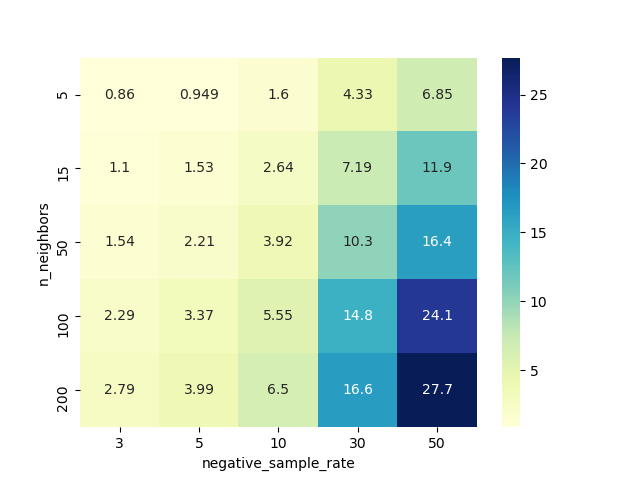
\includegraphics[width=4.5cm,height=4cm\textwidth]{images/umap/comparison/Digit_elapsed_time_n_neighbors_negative_sample_rate_heatmap.png}}
\centering
\caption{Running time for negative\_sample\_rate and n\_neighbors on Digits dataset with other parameters set to default}
% \label{Fig.main}
\end{figure}

% \begin{figure}[H]
% \centering  %图片全局居中
% \subfigure[$n\_neighbors$ and $spread$]
% {
% \label{Fig.sub.1}
% 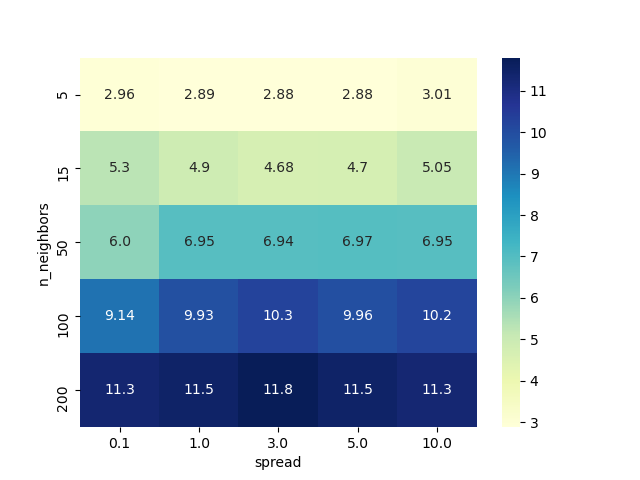
\includegraphics[width=7cm,height=4cm\textwidth]{images/umap/comparison/Digit_elapsed_time_n_neighbors_spread_heatmap.png}}
% \subfigure[$spread$ and $negative\_sample\_rate$]
% {
% \label{Fig.sub.2}
% 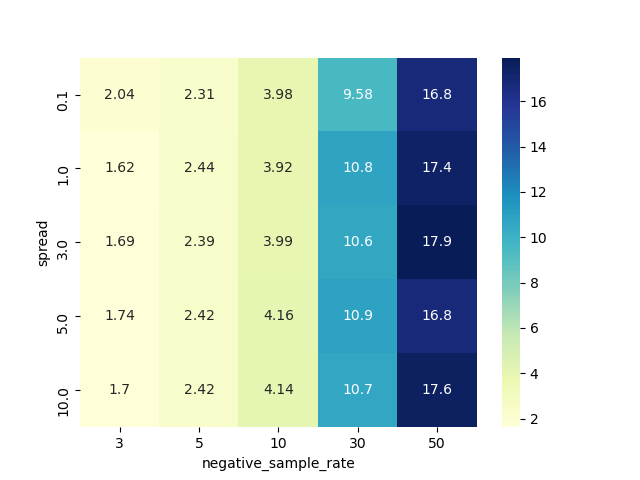
\includegraphics[width=7cm,height=4cm\textwidth]{images/umap/comparison/Digit_elapsed_time_spread_negative_sample_rate_heatmap.png}}
% \caption{Heatmap result with all the parameter pair in Digit dataset}
% % \label{Fig.main}
% \end{figure}

It is clear that $n\_neighbors$ and $negative\_sample\_rate$  play a major role in the increase of running time. When it comes to heatmap for $n\_neighbors$ and $negative\_sample\_rate$, the highest running time comes when these two parameters set to highest.

\end{enumerate}\\

\section{Largevis}

This experiment focuses on the four most important parameters of the Largevis algorithm. The basic ideas of them are:

\begin{enumerate}[1)]
\item $perp$: The perplexity used for deciding edge weights in KNN graph
\item $neg$: Number of negative samples used for negative sampling
\item $gamma$: The weights assigned to negative edges
\item $neigh$: Number of neighbors (K) in KNN graph, which is usually set as three times of perplexity
\end{enumerate}\\

\subsection{Installation and modification}

Because the Largeevis algorithm is not integrated in any python software package, but a series of C++ and python source codes are provided on github, it needs to be deployed before using the algorithm. \\

\noindent The C++ code needs to be compiled in the VS environment, so the first step is to download and configure Visual studio. Second, Since a large number of related library functions are used in the project, Boost must be configured in advance. The Boost library is a portable C++ library that provides source code. As a backup to the standard library, it is one of the development engines of the C++ standardization process.\\

\noindent In principle, the Largevis should be installed on the computer after two procedures. however, since the python code of the source code is based on python 2.7 and version on the computer is 3.7. Also the C++ code's version is different, there are some API do not use the previous names and the usage of some functions changed also. It is also necessary to modify the code base on the differences. 

\subsection{$perp$}

Since the approach to calculate conditional probability in HD and the weights of KNN graph is the same as t-SNE, the parameter $perplexity$ play the similar role, which is basically to maintain a balance between the local and global aspects of the data by deciding edge weights in building HD KNN graph. Here below are visualization results with different potential perplexity values on 6 datasets:

\begin{figure}[H]
\centering  %图片全局居中
% \subfigure[BCW]
{
\label{Fig.sub.1}
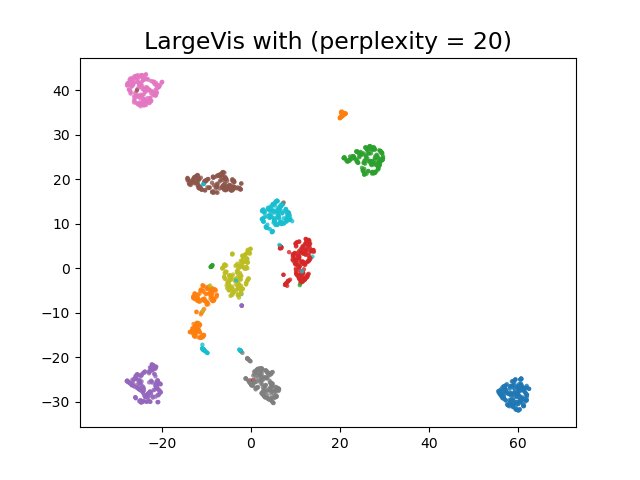
\includegraphics[width=7cm,height=4cm\textwidth]{images/largevis/image_largevis_perp20.png}}
% \subfigure[Oliv]
{
\label{Fig.sub.2}
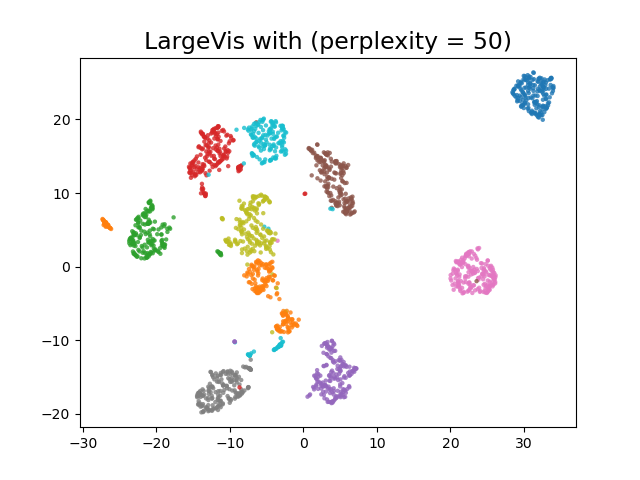
\includegraphics[width=7cm,height=4cm\textwidth]{images/largevis/image_largevis_perp50.png}}
% \caption{LD result for UMAP with n\_iter 50 and 200}
% \label{Fig.main}
\end{figure}

\begin{figure}[H]
\centering  %图片全局居中
% \subfigure[Digit]
{
\label{Fig.sub.1}
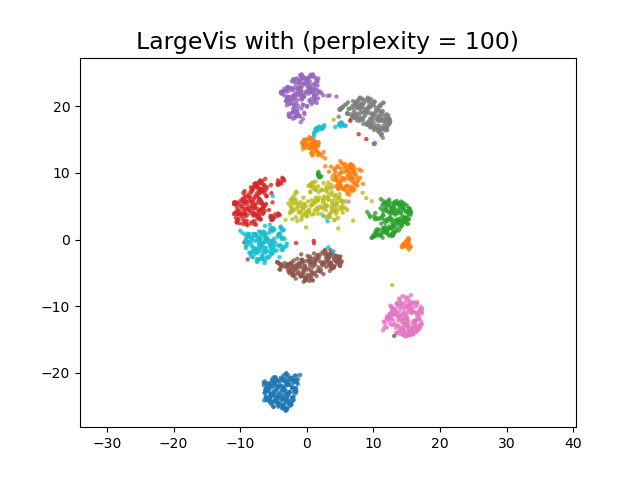
\includegraphics[width=7cm,height=4cm\textwidth]{images/largevis/image_largevis_perp100.png}}
% \subfigure[LFW]
{
\label{Fig.sub.2}
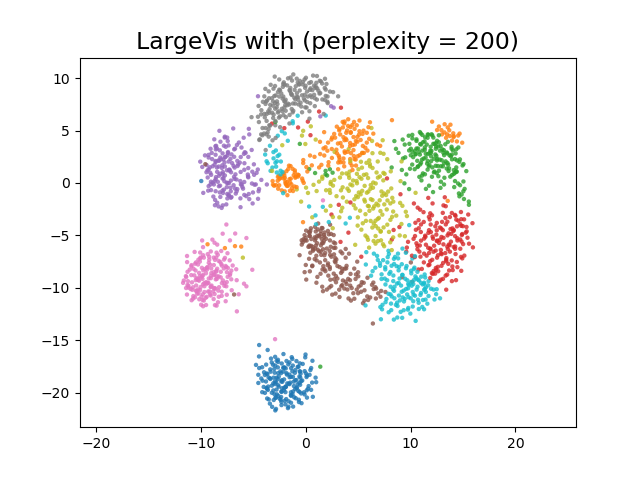
\includegraphics[width=7cm,height=4cm\textwidth]{images/largevis/image_largevis_perp200.png}}
\caption{LargeVis results with different Perplexity}
% \label{Fig.main}
\end{figure}

\noindent From the figure we can observe that when the $perplexity$ is 20 and 50, the clusters are well separated with a better global and local balance. While after 100, clusters start to merge. When $perplexity$ reach 200, the gap in between are blurry. The AUC value of them are 0.48, 0.487, 0.375, 0.383 separately because there are not the parameter $random_stateis$ in its source code, the values above are average score with 5 iterations for each considering that the algorithm are still using stochastic method.

\subsection{$neigh$}
As with the official Barnes-Hut t-SNE implementation, the LargeVis reference implementation uses a default perplexity of 50, and the default number of nearest neighbors is 3 times the perplexity. 

\subsection{$neg$}

As the key parameter for negative sampling in LD visualization part. $neg$ determine the number of negative samples used. Same as theoretical part, if we select samples an edge in the set of edges with the non-zero weight(E) such that $p_{ij} \neq 0$. This is called a “positive edge”. i and j are used to calculate the attractive part of the gradient. If we sample one of the N vertices($neg$). As datasets grow larger, the probability that $neg$ is in E grows smaller. Here below are visualization results with different potential perplexity values on Digits dataset: 

\begin{figure}[H]
\centering  %图片全局居中
% \subfigure[BCW]
{
\label{Fig.sub.1}
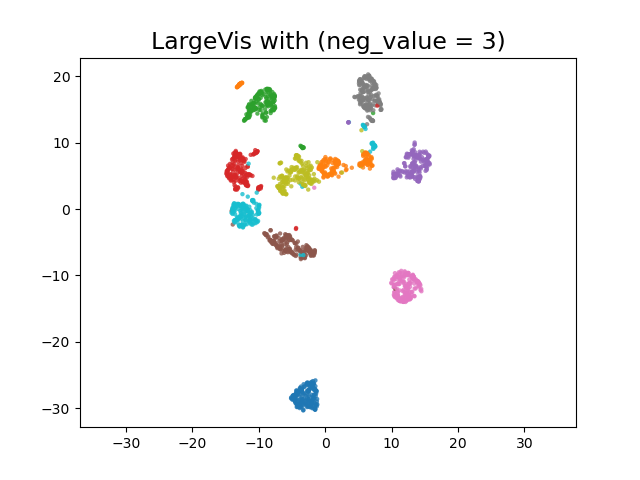
\includegraphics[width=7cm,height=4cm\textwidth]{images/largevis/image_largevis_neg3.png}}
% \subfigure[Oliv]
{
\label{Fig.sub.2}
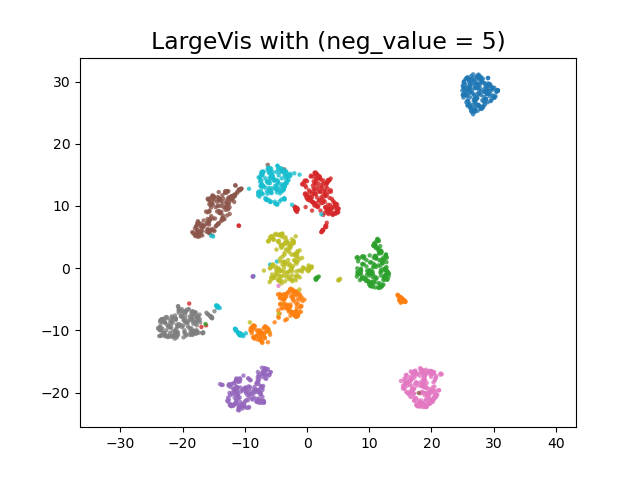
\includegraphics[width=7cm,height=4cm\textwidth]{images/largevis/image_largevis_neg5.png}}
% \caption{LD result for UMAP with n\_iter 50 and 200}
% \label{Fig.main}
% \end{figure}

% \begin{figure}[H]
\centering  %图片全局居中
% \subfigure[Digit]
{
\label{Fig.sub.1}
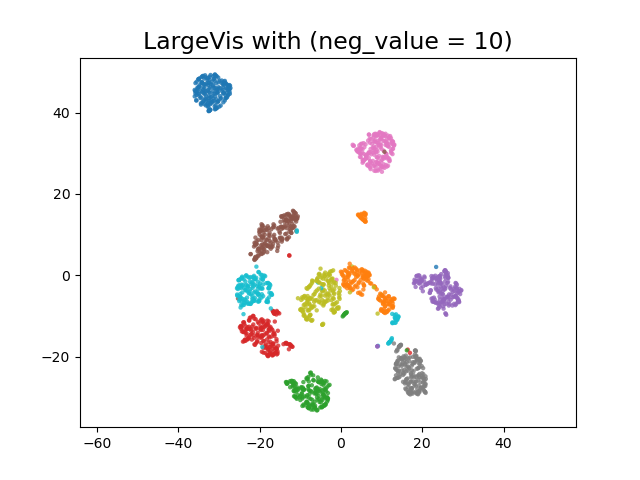
\includegraphics[width=7cm,height=4cm\textwidth]{images/largevis/image_largevis_neg10.png}}
% \subfigure[LFW]
{
\label{Fig.sub.2}
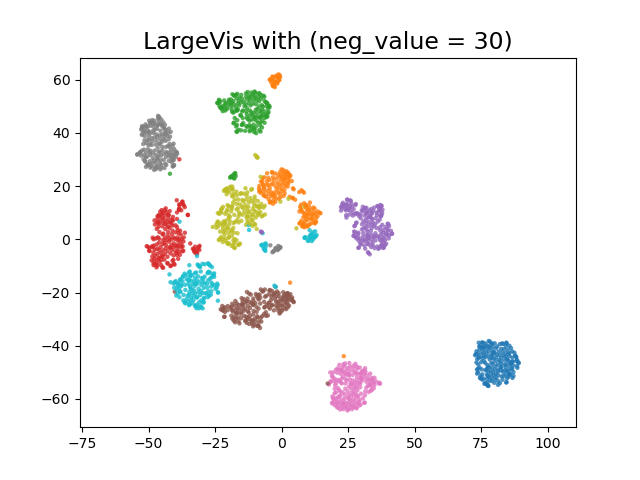
\includegraphics[width=7cm,height=4cm\textwidth]{images/largevis/image_largevis_neg30.png}}
\caption{LargeVis results with different neg}
% \label{Fig.main}
\end{figure}

\noindent As we can see from 6.13, the average distance between clusters increase as $neg$ variable increases. Their AUC values are 0.45, 0.46, 0.50, 0.51 separately. This is because the "repulsive force" of the cost function strengthened. At the same time, the time consumption is also added since the vertices of KNN graph it need to consider increased multiple times. 

\subsection{$gamma$}

$gamma$ stand for the weights assigned to negative edges. In the optimization process of Largevis, the goal is to maximize the probability that a positive sample node pair has a connected edge in the kNN graph, and minimize the probability that a negative sample node pair has a connected edge in the kNN graph, where $\gamma$ is the unified the weight set by the negative sample edge. Similar to the relationship between perp and neigh, $nag$ and $gamma$ set the number and weight of negative sample edges.

\subsection{relationships between algorithms and parameters}

% 1)

After observing the heatmap results, the two most important parameters for building KNN graph in HD and visualization algorithm in LD, have the greatest impact on AUC values. Here below are the relationships between them:

\begin{figure}[H]
\centering  %图片全局居中
\subfigure[BCW]
{
\label{Fig.sub.1}
\includegraphics[width=10cm,height=4cm\textwidth]{images/largevis/heatmap_perp_neg_BCW.png}}
\subfigure[Digits]
{
\label{Fig.sub.2}
\includegraphics[width=4.5cm,height=4cm\textwidth]{images/largevis/heatmap_perp_neg_Digits.png}}
% \caption{LD result for UMAP with n\_iter 2 and 15}
% \label{Fig.main}
\subfigure[LFW]
{
\label{Fig.sub.2}
\includegraphics[width=4.5cm,height=4cm\textwidth]{images/largevis/heatmap_perp_neg_LFW.png}}
% \caption{LD result for UMAP with n\_iter 2 and 15}
% \label{Fig.main}
\end{figure}

% \subsection{time consumption}

% It is easy to find that LargeVis sometimes consume more time than t-SNE during the examination procedure. 

% 1 最影响running time 的para


% 2 三个algos可以一起比一下,用default values
% 之后提出问题,why Largevis is slower than t-sne

\section{Visualization result with optimal parameters}

After examining all representative representative parameter values using grid search, the optimal parameter settings of each algorithm for each dataset are generated. The figure below shows the visualization results of each algorithm on the data set:


\begin{figure}[H]
\centering  %图片全局居中
\subfigure[t-SNE on Iris]
{
\label{Fig.sub.1}
\includegraphics[width=4.5cm,height=4cm\textwidth]{images/conclusion/t-SNE_Iris_0.759.png}}
\subfigure[UMAP on Iris]
{
\label{Fig.sub.2}
\includegraphics[width=4.5cm,height=4cm\textwidth]{images/conclusion/UMAP_Iris_0.749png.png}}
% \caption{LD result for UMAP with n\_iter 2 and 15}
% \label{Fig.main}
\subfigure[LargeVis on Iris]
{
\label{Fig.sub.2}
\includegraphics[width=4.5cm,height=4cm\textwidth]{images/conclusion/Largevis_Iris_0601.png}}
% \caption{LD result for UMAP with n\_iter 2 and 15}
% \label{Fig.main}
\end{figure}

\begin{figure}[H]
\centering  %图片全局居中
\subfigure[t-SNE on Wine]
{
\label{Fig.sub.1}
\includegraphics[width=4.5cm,height=4cm\textwidth]{images/conclusion/t-SNE_Wine_0.797.png}}
\subfigure[UMAP on Wine]
{
\label{Fig.sub.2}
\includegraphics[width=4.5cm,height=4cm\textwidth]{images/conclusion/UMAP_Wine_0.749png.png}}
% \caption{LD result for UMAP with n\_iter 50 and 200}
% \label{Fig.main}
\subfigure[LargeVis on Wine]
{
\label{Fig.sub.2}
\includegraphics[width=4.5cm,height=4cm\textwidth]{images/conclusion/Largevis_Wine_0577_plot.png}}
% \caption{LD result for UMAP with n\_iter 2 and 15}
% \label{Fig.main}
\end{figure}

\begin{figure}[H]
\centering  %图片全局居中
\subfigure[t-SNE on Oliv]
{
\label{Fig.sub.1}
\includegraphics[width=4.5cm,height=4cm\textwidth]{images/conclusion/t-SNE_Oliv_0.6.png}}
\subfigure[UMAP on Oliv]
{
\label{Fig.sub.2}
\includegraphics[width=4.5cm,height=4cm\textwidth]{images/conclusion/UMAP_Oliv_0.536.png}}
% \caption{LD result for UMAP with n\_iter 2 and 15}
% \label{Fig.main}
\subfigure[LargeVis on Oliv]
{
\label{Fig.sub.2}
\includegraphics[width=4.5cm,height=4cm\textwidth]{images/conclusion/Largevis_Oliv_0576_plot.png}}
% \caption{LD result for UMAP with n\_iter 2 and 15}
% \label{Fig.main}
% \end{figure}

% \begin{figure}[H]
\centering  %图片全局居中
\subfigure[t-SNE on BCW]
{
\label{Fig.sub.1}
\includegraphics[width=4.5cm,height=4cm\textwidth]{images/conclusion/t-SNE_BCW_0.768.png}}
\subfigure[UMAP on BCW]
{
\label{Fig.sub.2}
\includegraphics[width=4.5cm,height=4cm\textwidth]{images/conclusion/UMAP_BCW_0.713.png}}
% \caption{LD result for UMAP with n\_iter 50 and 200}
% \label{Fig.main}
\subfigure[LargeVis on BCW]
{
\label{Fig.sub.2}
\includegraphics[width=4.5cm,height=4cm\textwidth]{images/conclusion/Largevis_BCW_0731_plot.png}}
% \caption{LD result for UMAP with n\_iter 2 and 15}
% \label{Fig.main}
% \end{figure}

% \begin{figure}[H]
\centering  %图片全局居中
\subfigure[t-SNE on Digits]
{
\label{Fig.sub.1}
\includegraphics[width=4.5cm,height=4cm\textwidth]{images/conclusion/t-SNE_Digits_0.55.png}}
\subfigure[UMAP on Digits]
{
\label{Fig.sub.2}
\includegraphics[width=4.5cm,height=4cm\textwidth]{images/conclusion/UMAP_Digits_0.499.png}}
% \caption{LD result for UMAP with n\_iter 50 and 200}
% \label{Fig.main}
\subfigure[LargeVis on Digits]
{
\label{Fig.sub.2}
\includegraphics[width=4.5cm,height=4cm\textwidth]{images/conclusion/Largevis_Digits_0468_plot.png}}
% \caption{Visualization results on 6 datasets}
% \label{Fig.main}
\end{figure}

\begin{figure}[H]
\centering  %图片全局居中
\subfigure[t-SNE on LFW]
{
\label{Fig.sub.1}
\includegraphics[width=4.5cm,height=4cm\textwidth]{images/conclusion/t-SNE_LFW_0.359.png}}
\subfigure[UMAP on LFW]
{
\label{Fig.sub.2}
\includegraphics[width=4.5cm,height=4cm\textwidth]{images/conclusion/UMAP_LFW_0.324.png}}
% \caption{LD result for UMAP with n\_iter 50 and 200}
% \label{Fig.main}
\subfigure[LargeVis on LFW]
{
\label{Fig.sub.2}
\includegraphics[width=4.5cm,height=4cm\textwidth]{images/conclusion/Largevis_LFW_0332_plot.png}}
\caption{Visualization results on 6 datasets}
% \label{Fig.main}
\end{figure}

\noindent We can see that on the smallest data set with houndreds of instances and dimensions, like Iris, Wine and BCW, the visualization images generated by t-SNE, UMAP and LargeVis are both meaningful and can be compared with each other. \\

\noindent However, when it comes to the image dataset, like Oliv(with N = 400, M = 1096) and LFW(with N = 13233 , M = 5749 ), all three algorithms do not have a good performance. At the same time, the outcome of Digits dataset(with N = 1797, M = 64), which is also a image dataset, identify the clusters clearly. This may because the image of the first two datasets are consist of houndreds of objects at different angles, after transforming them into pixels, the image of same object at different angle could be regarded as different clusters. The following chart and table show the AUC values and time consumption on each dataset of three algorithms with optimal parameters:\\
\\

\begin{figure}[ht]

\centering
\includegraphics[width=12cm,height=5cm\textwidth]{images/conclusion/AUC_result.PNG}
\caption{AUC values for each dataset of algorithms with optimal parameters}
\label{fig:label}
\end{figure}\\

\begin{table}[h]  %table 里面也可以嵌套tabular,只有tabular是不能加标题的
\centering  %表格居中
 %表格标题
 \begin{tabular}{|c|c|c|c|}  %右对齐
    %  \hline
     \hline
       Datasets & t-SNE & UMAP & LargeVis\\
       [0.5ex]  %增加行宽
      
        \hline  %在第一行和第二行之间绘制横线
        Iris(N=150,M=4) & 2.89 & 1.37 & 408.15\\
        \hline  %在第一行和第二行之间绘制横线
        Wine(N=178,M=13) & 5.55 & 1.43 & 414.15\\
        \hline  %在第一行和第二行之间绘制横线
        Oliv(N=400,M=4096) & 18.65 & 4.4 & 427.23\\
        \hline  %在第一行和第二行之间绘制横线
        BCW(N=569,M=30) & 23.15 & 5.39 & 425.95\\
        \hline  %在第一行和第二行之间绘制横线
        Digits(N=1797,M=64) & 49.01 & 9.23 & 535.71\\
        \hline  %在第一行和第二行之间绘制横线
        LFW(N=13233,M=5749) & 1181.07 & 98.18 & 1625.84\\
    %   \hline
    %   \multicolumn{2}{c}{Total Sqerr} & 10.12 & 8.13 \\  %横向合并两个单元格
       \hline
    %   \hline
   \end{tabular}
   \caption{Time consumption for each dataset of algorithms with optimal parameters} 
\end{table}\\
% 可以画一个不同dataset上的散点图
\\
\\
\noindent From the all the results, we can find out that:\\

\begin{enumerate}[1)]
\item The number of dimension does not really matters the running time.
\item The AUC score of t-SNE and Largevis with optimal parameters are almost the same with always 1 to 2 percent of difference. However, the AUC score of UMAP always has less 7 to 8 percent. 
% \item The parameters vary less strong from dataset to dataset comparing to two other algorithm, which means 
\item Considering the following time consumption and LD results above, we can draw the conclusion that when it is needed to have a fast result or better understanding of global structure of HD data, the UMAP is the best choice. If the result need to be more accurate and more attention to details of the structure in HD, when the instances of the dataset is less than $10^5$ level, t-SNE will save more time. When it is above, LargeVis is the better one with less time consumption\cite{ref5}.
\end{enumerate}\\

% 可以画一个不同dataset上的散点图
\chapter{Conclusion}

This thesis studies the three most advanced data dimensionality reduction algorithms based on random neighbor embedding methods, namely t-SNE, UMAP and LargeVis. This article first derives three algorithms from the perspective of theory and experiment. The DR quality standard is also used to measure the performance of the three algorithms on different data sets. Then, check the more important parameters of each algorithm, and similar variables of different algorithms, and explore the possible reasons that lead to their different results. Finally, the grid search algorithm is used to measure the best variables of the three DR algorithms, and the similarities and differences of the algorithms running under the best conditions are compared. Experiments on actual data sets show that UMAP has better running time and retention of global structure, while LargeVis has better quality of local visualization results. Although t-SNE focus almost only on the local structure, the best parameter performance of its AUC value is at the same level as the other two algorithms. In the future, inspired by the neural network structure of the autoencoder, its middle layers will be compared horizontally, and the comparison dimension will be expanded from 2 dimensions to multiple dimensions.


% 重新组织一下结构,先说Qnx,再说Rnx,最后说AUC,和其值代表的意义。
